\subsection{Problem 4}%
\label{sec:problem_4}
Using least squares find the ``best'' straight-line fit and the error estimates for the
slope and intercept of that line for the following set of data:
\begin{center}
  \begin{tabular}{|c|c|c|c|c|c|c|c|c|}
    \hline
    $x_i$ & 1 & 2 & 3 & 4 & 5 & 6 & 7 & 8 \\
    \hline
    $y_i$ & 1.5 & 2.0 & 2.8 & 4.1 & 4.9 & 6.3 & 5.0 & 11.5 \\
    \hline
  \end{tabular}
\end{center}
%%%%%%%%%%%%%%%%%%%%%%%%%%%%%%%%%%%%%%%%%%%%%%%%%%%%%%%%%%%%%%%%%%%%%%%%%%%%%%%
\subsubsection*{Mathematics}
%%%%%%%%%%%%%%%%%%%%%%%%%%%%%%%%%%%%%%%%%%%%%%%%%%%%%%%%%%%%%%%%%%%%%%%%%%%%%%%
We want to fit the data above to the function in the form $y = a_0 + a_1x$.
We may proceed with this problem just as in the previous ones.

We may also find the solution with the \textit{linear regression} approach.
Following~\cite{Zdunek}, the least-squares solution defining the best-fitting line
$y = a_0 + a_1x$ to the set of points $(x_i, y_i)$ for $i=1,\ldots,M$ may be derived from
the normal equations:
\begin{equation*}
a_1 = \frac{\sum_{i=1}^M{y_i x_i}-M\bar{y}\bar{x}}{\sum_{i=1}^M{x_i^2}-M\bar{y}\bar{x}}
\qquad a_0 = \bar{y} - a_1\bar{x}
\end{equation*}
which is implemented in the~\nameref{algorithm:2}.

Additionally, we may calculate the linear regression error $\varepsilon$:
\begin{equation*}
  \varepsilon = \left\lVert\matr{b}-\matr{A}\matr{x}\right\rVert_2^2
\end{equation*}
which for this problem is simply:
\begin{equation*}
  \varepsilon = \sum_{i=1}^M{{\left(y_i-a_0-a_1x_i\right)}^2}
\end{equation*}
%%%%%%%%%%%%%%%%%%%%%%%%%%%%%%%%%%%%%%%%%%%%%%%%%%%%%%%%%%%%%%%%%%%%%%%%%%%%%%%
\subsubsection*{Solution}
%%%%%%%%%%%%%%%%%%%%%%%%%%%%%%%%%%%%%%%%%%%%%%%%%%%%%%%%%%%%%%%%%%%%%%%%%%%%%%%
The two approaches presented above give us very similar results:
\lstinputlisting[style=Matlab-editor]{problems/Problem_4.m}
for which the plot may be seen in the~\autoref{fig:problem_4}.
\begin{figure}
  \centering
  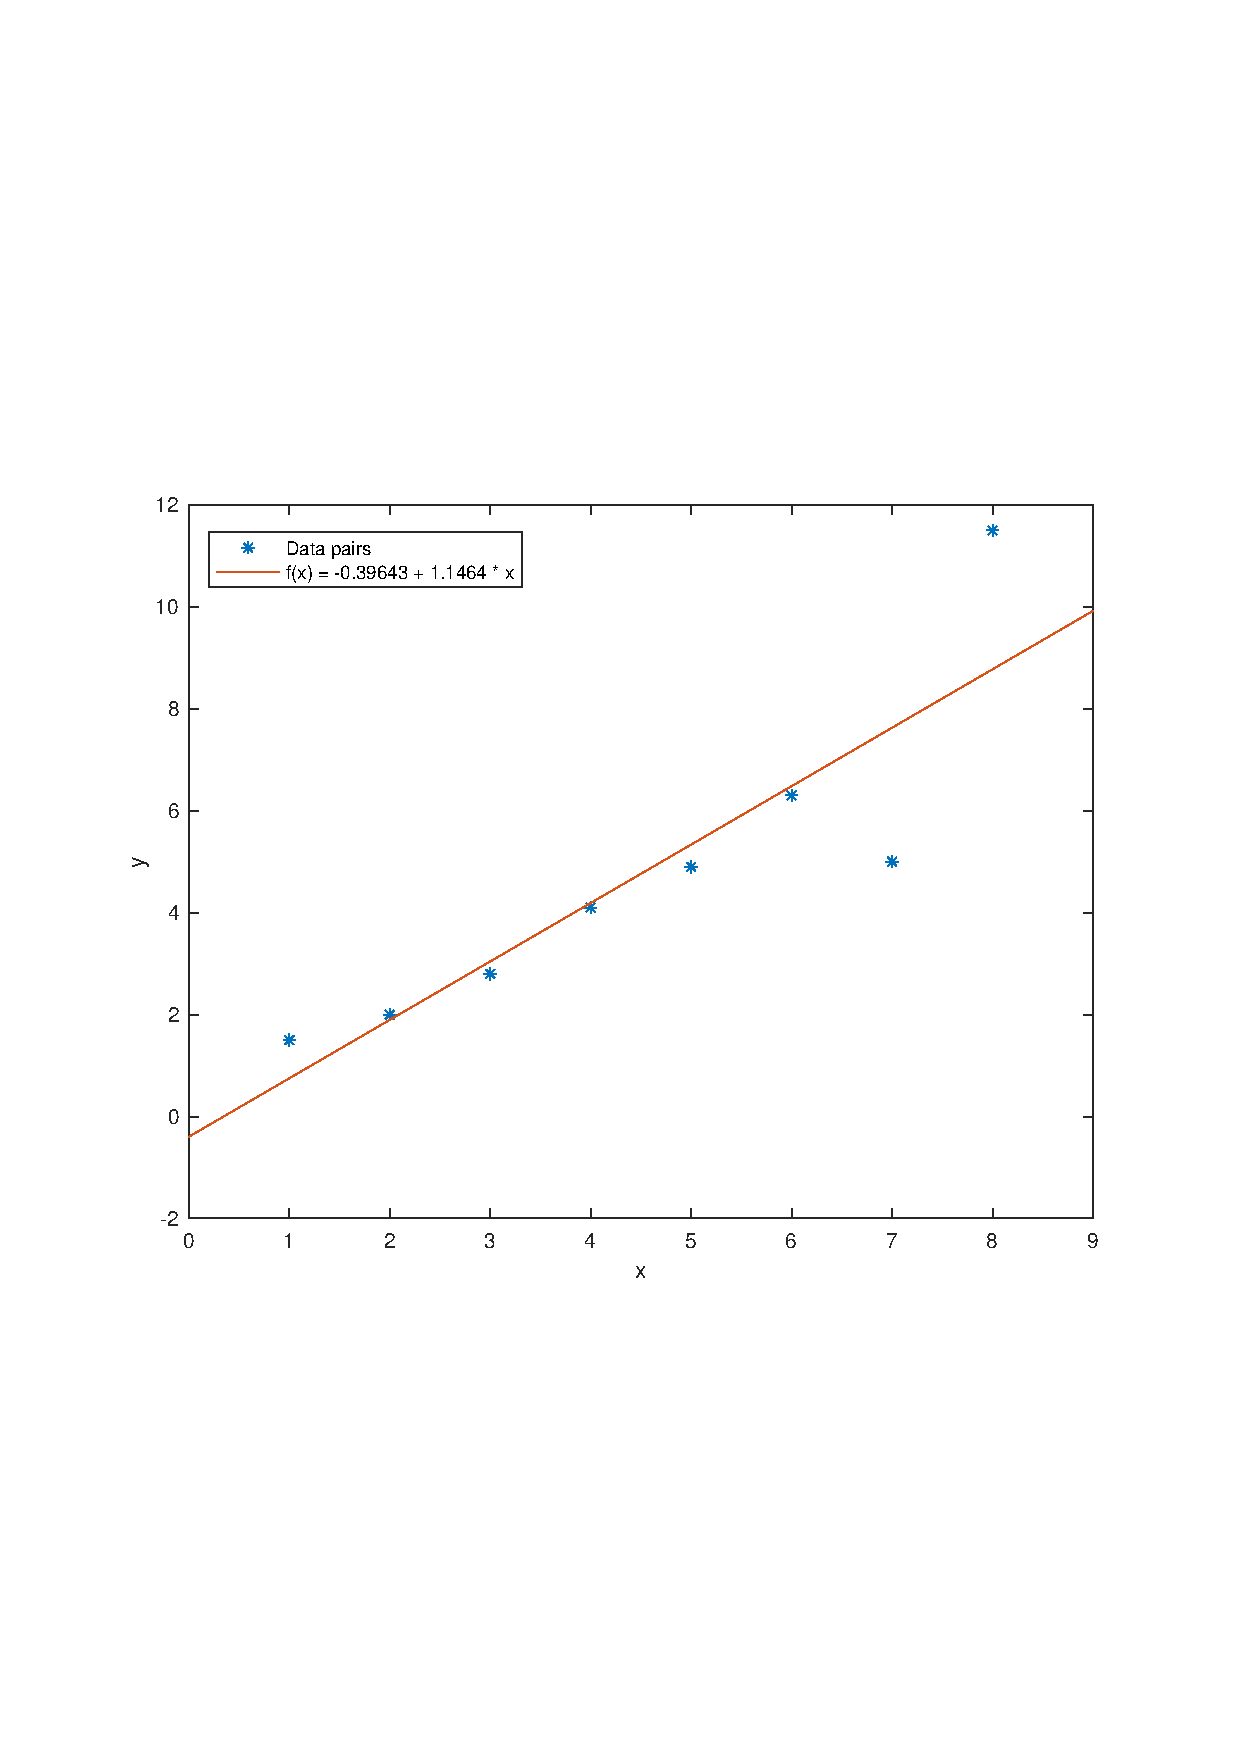
\includegraphics[width=0.7\textwidth]{images/Problem_4_plot.pdf}
  \caption{The plot of the approximated solution and predefined data pairs
    for the Problem~4}\label{fig:problem_4}
\end{figure}
